%Motivacia, ine vysledky
%Ohurit komisiu
%Urobili vela prace, Nebolo to lahke


\documentclass[xcolor=dvipsnames, compress, 12pt]{beamer} 
\usepackage[utf8]{inputenc}
\usepackage[slovak]{babel}
\usepackage{lmodern}
\usepackage[T1]{fontenc}
\usepackage{amsfonts}
\usepackage{amssymb}
\usepackage{amsthm}
\usepackage{amsmath}
\usepackage{epsfig}
\usepackage{wrapfig}
\usepackage{caption}
\usepackage{subcaption}
\usepackage{url}
\usepackage{hyperref}
% \usepackage{multicol}
\usecolortheme[named=Green]{structure} 
\usetheme{Dresden} 
\setbeamertemplate{navigation symbols}{}
\usebackgroundtemplate{
\includegraphics[width=\paperwidth, height=\paperheight]{images/bg.png}}
% \setbeamertemplate{footline}[frame number]
% \setbeamertemplate{items}[ball] 
% \setbeamertemplate{blocks}[rounded][shadow=true] 
% \useoutertheme{umbcfootline} 

% \AtBeginSection[]{
% \frame<beamer>{
  
%     \ifpdf
%       \pdfbookmark[0]{Contents}{toc}
%     \fi    
%     \frametitle{Obsah}
%     \setcounter{tocdepth}{2}      
%     \tableofcontents[currentsection,subsections,hideothersubsections]
  
% }
% }

% Show frame number in footbar
\setbeamertemplate{footline}%{miniframes theme}
  {%
    \begin{beamercolorbox}[colsep=1.5pt]{upper separation line foot}
    \end{beamercolorbox}
    \begin{beamercolorbox}[ht=2.5ex,dp=1.125ex,%
      leftskip=.3cm,rightskip=.3cm plus1fil]{author in head/foot}%
      \leavevmode{\usebeamerfont{author in head/foot}\insertshortauthor}%
      \hfill%
      {\usebeamerfont{institute in head/foot}\usebeamercolor[fg]{institute in head/foot}\insertshortinstitute}%
    \end{beamercolorbox}%
    \begin{beamercolorbox}[ht=2.5ex,dp=1.125ex,%
      leftskip=.3cm,rightskip=.3cm plus1fil]{title in head/foot}%
      {\usebeamerfont{title in head/foot}\insertshorttitle} \hfill     \insertframenumber /\inserttotalframenumber % 
    \end{beamercolorbox}%
    \begin{beamercolorbox}[colsep=1.5pt]{lower separation line foot}
    \end{beamercolorbox}
  }

% items enclosed in square brackets are optional; explanation below
\title{Zarovnávanie sekvencií s použitím metód klasifikácie}
\subtitle{
\vspace{0.5cm}
\small Diplomová práca
}
\author[Michal Hozza]{\small Bc. Michal Hozza \\ \vspace{1cm} \footnotesize \textbf{Vedúci práce:} Mgr. Tomáš Vinař, PhD. \\ \textbf{Konzultant:} Mgr. Michal Nánási\\ \vspace{.5cm}}
\institute[FMFI UK \insertshortdate]{
  Fakulta matematiky, fyziky a informatiky,
  Univerzita Komenského, Bratislava\\
}
\date[\the\year]{\footnotesize \today}

\begin{document}

%--- the titlepage frame -------------------------%
\begin{frame}[plain]
  \titlepage
\end{frame}

%--- the presentation begins here ----------------%

\begin{frame}{Obsah}
  \transdissolve[duration=0.1]
  \tableofcontents
\end{frame}


\section{Úvod}
\subsection{Cieľ}
\begin{frame}{Cieľ}
  % \transdissolve
  \begin{itemize}
  \item Cieľom práce je vytvoriť nové metódy na korekciu zarovnaní biologických sekvencií na základe prídavnej informácie.
  \item Integrácia tejto informácie bude zabezpečená pomocou techník využívaných na klasifikáciu v strojovom učení.
  \end{itemize} 
\end{frame}


\subsection{Zarovnávanie sekvencií}
\begin{frame}{Zarovnávanie sekvencií}
Kľúčové problémy:
  \begin{itemize}
    \pause
    \item Aké typy zarovnávania by sme mali uvažovať
    \pause
    \item Skórovací systém, ktorý použijeme na ohodnotenie zarovnania a trénovanie
    \pause
    \item Algoritmus, ktorý použijeme na hľadanie optimálneho alebo dobrého zarovnania podľa skórovacieho systému
    \pause
    \item Štatistická významnosť zarovnania.
  \end{itemize} 
\end{frame}

\section{Modely a Existujúce riešenia}
\subsection{Modely}
\begin{frame}{Modely}
Generatívny:
\begin{itemize}
\item sa snaží modelovať proces, ktorý generuje dáta ako pravdepodobnosť $P(X,Y,Z)$
\item rozložíme ju pomocou nezávislých predpokladov na procese $\longrightarrow$ obmedzujúce
\end{itemize} 
\pause
Diskriminačný
\begin{itemize}
\item priamo odhaduje $P(Z|X,Y)$ alebo prislúchajúcu diskriminačnú funkciu, a preto sa zamerá na podstatnú časť problému odhadu
\item Nepotrebuje nezávislosť $\longrightarrow$ silnejšie
\end{itemize}   
\end{frame}


% \subsection{Existujúce riešenia}
% \begin{frame}{Existujúce riešenia}
%   \begin{itemize}
%     \item Problém inverzného zarovnania
%     \pause
%     \item Support vector training of protein alignment models
%     \begin{itemize}
%       \item Support Vector Machine (SVM)
%       \item Umožňuje trénovať pomocou rôznych účelových funkcií
%     \end{itemize}
%     \pause
%     \item Contralign: Discriminative training for protein sequence alignment.
%     \begin{itemize}
%       \item Conditional Random Fields (CRF)
%       \item Neumožnuje trénovať pomocou rôznych účových funkcií    
%     \end{itemize}
%   \end{itemize} 
% \end{frame}

\section{Naše riešenie}
% \subsection{Odlišnosti nášho riešenia}
% \begin{frame}{Odlišnosti nášho riešenia}
%   \begin{itemize}
%     \item Korekcia existujúcich zarovnaní
%     \begin{itemize}
%       \item Použitie súbežne s existujúcimi zarovnávačmi
%     \end{itemize}
%     \pause
%     \item Rôzne metódy trénovania
%     \pause
%     \item Možnosť učenia bez učiteľa
%     \pause
%     \item Iný klasifikátor
%     \begin{itemize}
%       \item možno porovnanie viac rôznych klasifikátorov
%       \item pípadne abstrakcia od klasifikátora
%     \end{itemize} 
%   \end{itemize} 
% \end{frame}

\subsection{Základný model}
\begin{frame}{Základný model}
  \begin{itemize}
    \item 3 stavový HMM
    \begin{itemize}
      \item Match
      \item Insert X
      \item Insert Y
    \end{itemize} 
    \pause
    \item Viterbiho algoritmus
    \begin{itemize}
      \item pravdepodobnosti získané z natrénovaného klasifikátora
	\end{itemize}    
	\pause
	\item rozšírenie sekvencií o anotácie
  \end{itemize} 
\end{frame}


% \subsection{Klasifikátor}
% \begin{frame}{Klasifikátor}
% Random Forest
%   \begin{itemize}
%     \item Zložený z klasifikačných (rozhodovacích) stromov
%     \item Stromy hlasujú o výsledku
%   \end{itemize} 
%   \vspace{.5cm}
%   \begin{center}
%   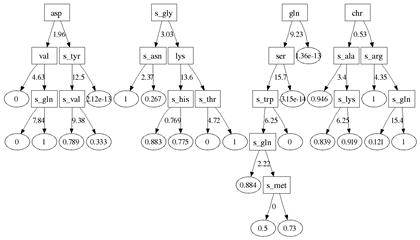
\includegraphics[width=.5\textwidth]{images/random_forest_thumb.png}
%   \end{center}
% \end{frame}

\subsection{Simulátor}
\begin{frame}{Simulátor}
  \begin{itemize}
    \item Model určený na prvotné experimenty
    \item Program simuluje evolúciu
    \begin{itemize}
      \item Generovanie dvojice postupností so správnym zarovnaním
      \item Generovanie dodatočej informácie
      \item Simulácia mutácie a delécie
    \end{itemize} 
  \end{itemize} 
\end{frame}

\section{Experimenty}
\subsection{Simulované dáta}
\begin{frame}{Dodatočné informácie}  
  \begin{itemize}
    \item Stopa s informáciou, či daná pozícia je súčasťou génu
    \item Ukazuje sa, že dodatočné informácie dokážu pomôcť klasifikátoru v lepšej klasifikácii`
  \end{itemize} 
\end{frame}

\begin{frame}{Dodatočné informácie}  
\begin{figure}[hbtp]
    \centering
    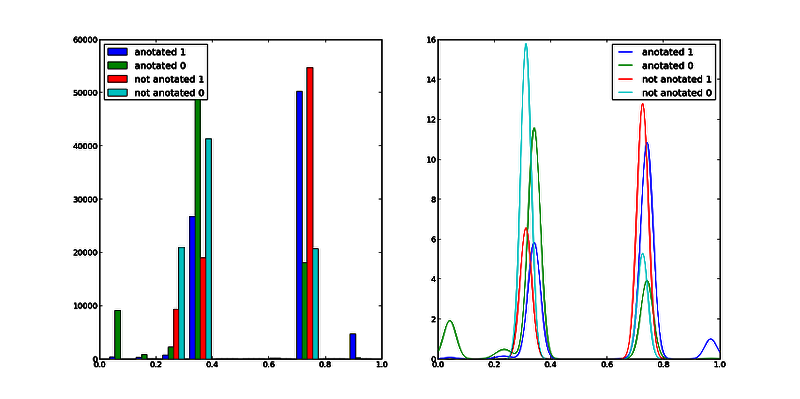
\includegraphics[width=\textwidth]{images/porovnanie_s1w1testset.png}
    \caption{Porovnanie distribúcie pravdepodobností bez anotácie a s anotáciou (100000 báz, okno veľkosti 1, testovacia množina)}    
    \label{fig:porovnanie_s1w1testset.png} 
\end{figure}
\end{frame}

\begin{frame}{Väčšie okno}  
  \begin{itemize}
    \item Väčšie okno sa prejaví vo väčšom množstve \textit{vlastností}, čo 
    \item Pri malom množstve doplnkovej informácie má výrazný vplyv 
    \item Pri väčšom množstve doplnkovej informácie ich znásobuje
  \end{itemize} 
\end{frame}

\begin{frame}{Väčšie okno}  
\begin{figure}[hbtp]
    \centering
    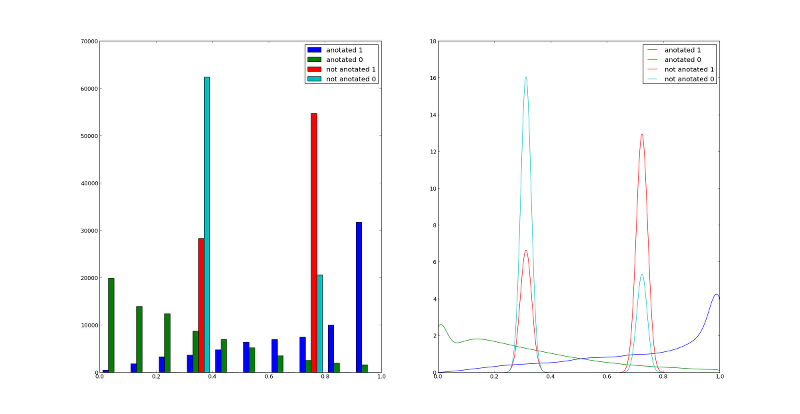
\includegraphics[width=0.9\textwidth]{images/porovnanie_s1w5vsw1testset.png}
    \caption{Porovnanie distribúcie pravdepodobností bez anotácie a oknom veľkosti 1 a s anotáciou s oknom veľkosti 5 (100000 báz, testovacia množina)}
    \caption{s1w5vsw1testset}    
    \label{fig:porovnanie_s1w5vsw1testset.png} 
\end{figure}
\end{frame}


\section{}
\begin{frame}[plain]
  \transdissolve[duration=5]
  \begin{center}
  \textbf{\color{Green} \LARGE Ďakujem za pozornosť!} 
  \end{center}  
\end{frame}


\end{document}
